\documentclass{article}
\usepackage{CJKutf8}
\usepackage{amsmath}
\usepackage{amsfonts}
\usepackage{amsthm}
\usepackage{titlesec}
\usepackage{titletoc}
\usepackage{xCJKnumb}
\usepackage{tikz}
\usepackage{ragged2e}
\justifying\let\raggedright\justifying
  % \renewcommand{\chaptermark}[1]{\markboth{第 \thechapter 章}{}}
\usepackage{mathrsfs}

\newtheorem{Def}{定义}
\newtheorem{Thm}{定理}
\newtheorem{Exercise}{练习}
\newtheorem{Cor}{推论}

\newtheorem*{Example}{例}


\begin{document}
\begin{CJK*}{UTF8}{gbsn}
  \title{第二章映射}
  \author{陈建文}
  \maketitle
  % \tableofcontents
  

  \begin{Def}
    设$X$和$Y$为两个集合。一个从$X$到$Y$的{\bfseries 映射}$f$为一个法则,根据$f$,对$X$中的每个元素$x$都有$Y$中唯一确定的元素$y$与之对应。
    从$X$到$Y$的映射$f$常记为$f:X\to Y$。
  \end{Def}

  \begin{Example}
    设集合$X=\{-1,0,1\}$,集合$Y=\{0,1,2\}$,$\forall x \in X, f(x)=x^2$,即$f(-1)=1,f(0)=0,f(1)=1$,则$f$为从集合$X$到集合$Y$的映射。
  \end{Example}

  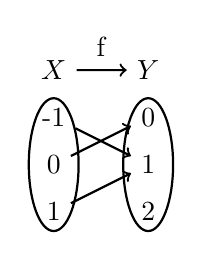
\begin{tikzpicture}[thick, scale=0.3]
  \draw (-2,0) ellipse [x radius=30pt, y radius=80pt];
  \draw (2,0) ellipse [x radius=30pt, y radius=80pt];
  \node[thick] (A) at (-2, 4) {$X$};
  \node[thick] (B) at (2,4) {$Y$};
  \draw[thick, ->] (A) to  (B);

  
  \node[thick] (C) at (-2,2) {-1};
   \node[thick] (D) at  (2,2) {0};

  
  \node[thick] (E) at (-2,0) {0};
  \node[thick] (F) at (2,0) {1};

    \node[thick] (G) at (-2,-2) {1};
    \node[thick] (H) at (2,-2) {2};

    
\draw[thick, ->] (C) to  (F);
\draw[thick, ->] (E) to  (D);
\draw[thick, ->] (G) to  (F);

\draw (0,5) node {f};
\end{tikzpicture}
  
  \begin{Def}
    设$X$和$Y$为两个集合。一个从$X$到$Y$的{\bfseries 映射}为一个满足以下两个条件的$X\times Y$的子集$f$:
    \begin{enumerate}
    \item 对$X$的每一个元素$x$,存在一个$y\in Y$,使得$(x,y) \in f$;
    \item 若$(x,y)\in f$,$(x,y')\in f$,则$y=y'$。
    \end{enumerate}
    $(x,y)\in f$记为$y=f(x)$。
  \end{Def}
  \begin{Example}
    设集合$X=\{-1,0,1\}$,集合$Y=\{0,1,2\}$,$f\subseteq X \times Y$,$f=\{(-1,1),(0,0),(1,1)\}$,则$f$为从集合$X$到集合$Y$的映射。
  \end{Example}

  定义2.1和定义2.2是等价的。

    \begin{Exercise}
    设$X=\{0,1,2\}, Y= \{3,4,5\}, f\subseteq X \times Y$,则下列为映射的是(D)

    A. $f = \{(0,3), (1,4)\}$

    B. $f = \{(0,3), (0,4), (1,4),(2,5)\}$

    C. $f = \{(0,3), (0,4)\}$

    D. $f = \{(0,5), (1,4), (2,3)\}$
  \end{Exercise}

   映射定义的符号化表示:

  $f:X\to Y$
  
  $f\subseteq X\times Y$

  1) $\forall x \in X \exists y\in Y (x,y) \in f$

  即:$\forall x x \in X \to \exists y y\in Y \land (x,y) \in f$

  2) $\forall x \in X \forall y \in Y \forall y'\in Y ((x,y) \in f \land (x, y') \in f \to y = y')$

  即:$\forall x x \in X \to (\forall y y \in Y \to \forall y' y' \in Y \to ((x,y) \in f \land (x, y') \in f \to y = y'))$
    
 
  \begin{Def}
    设$f$为从集合$X$到集合$Y$的映射,$f:X\to Y$, 如果$y = f(x)$,则称$y$为$x$在$f$下的{\bfseries 象},称$x$为$y$的{\bfseries 原象}。$X$称为$f$的{\bfseries 定义域};集合$\{f(x) | x \in X\}$称为$f$的{\bfseries 值域},记为$Im(f)$。
  \end{Def}

  P(x):x为偶数

$P:Z\to \{T,F\}$

$P\subseteq Z \times \{T,F\}$

$P=\{\ldots, (-2, T), (-1, F), (0, T), (1,F), (2,T), \ldots\}$


  \begin{Def}
    设$f:X\to Y$,$A\subseteq X$,当把$f$的定义域限制在$A$上时,就得到了一个
    $\phi: A\to Y$,$\forall x \in A$,$\phi(x) = f(x)$。$\phi$称为$f$在$A$上的
    限制,并且常用$f|A$来表示$\phi$。反过来,我们也称$f$为$\phi$在$X$上的扩张。
  \end{Def}


    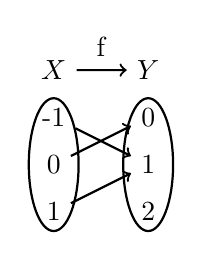
\begin{tikzpicture}[thick, scale=0.3]
  \draw (-2,0) ellipse [x radius=30pt, y radius=80pt];
  \draw (2,0) ellipse [x radius=30pt, y radius=80pt];
  \node[thick] (A) at (-2, 4) {$X$};
  \node[thick] (B) at (2,4) {$Y$};
  \draw[thick, ->] (A) to  (B);

  
  \node[thick] (C) at (-2,2) {-1};
   \node[thick] (D) at  (2,2) {0};

  
  \node[thick] (E) at (-2,0) {0};
  \node[thick] (F) at (2,0) {1};

    \node[thick] (G) at (-2,-2) {1};
    \node[thick] (H) at (2,-2) {2};

    
\draw[thick, ->] (C) to  (F);
\draw[thick, ->] (E) to  (D);
\draw[thick, ->] (G) to  (F);

\draw (0,5) node {f};
\end{tikzpicture}

    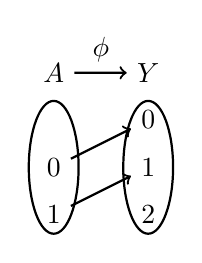
\begin{tikzpicture}[thick, scale=0.3]
  \draw (-2,0) ellipse [x radius=30pt, y radius=80pt];
  \draw (2,0) ellipse [x radius=30pt, y radius=80pt];
  \node[thick] (A) at (-2, 4) {$A$};
  \node[thick] (B) at (2,4) {$Y$};
  \draw[thick, ->] (A) to  (B);

  
%  \node[thick] (C) at (-2,2) {-1};
   \node[thick] (D) at  (2,2) {0};

  
  \node[thick] (E) at (-2,0) {0};
  \node[thick] (F) at (2,0) {1};

    \node[thick] (G) at (-2,-2) {1};
    \node[thick] (H) at (2,-2) {2};

    
%\draw[thick, ->] (C) to  (F);
\draw[thick, ->] (E) to  (D);
\draw[thick, ->] (G) to  (F);

\draw (0,5) node {$\phi$};
\end{tikzpicture}

    \begin{Def}
    设$f:A \to Y$,$A \subseteq X$, 则称$f$为$X$上的一个部分映射。
  \end{Def}
  一个部分映射的例子:
  
  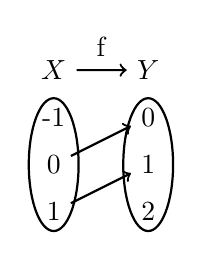
\begin{tikzpicture}[thick, scale=0.3]
  \draw (-2,0) ellipse [x radius=30pt, y radius=80pt];
  \draw (2,0) ellipse [x radius=30pt, y radius=80pt];
  \node[thick] (A) at (-2, 4) {$X$};
  \node[thick] (B) at (2,4) {$Y$};
  \draw[thick, ->] (A) to  (B);

  
  \node[thick] (C) at (-2,2) {-1};
   \node[thick] (D) at  (2,2) {0};

  
  \node[thick] (E) at (-2,0) {0};
  \node[thick] (F) at (2,0) {1};
  \draw[thick, ->] (E) to  (D);

    \node[thick] (G) at (-2,-2) {1};
    \node[thick] (H) at (2,-2) {2};
      \draw[thick, ->] (G) to  (F);
\draw (0,5) node {f};
\end{tikzpicture}
  \begin{Def}
    两个映射$f$与$g$称为是相等的当且仅当$f$和$g$都为从$X$到$Y$的映射,并且$\forall x \in X$总有$f(x) = g(x)$。
  \end{Def}
  \begin{Def}
    设$f:X\to X$,如果$\forall x \in X, f(x) = x$,则称$f$为$X$上的恒等映射。$X$上的恒等映射常记为$I_X$。
  \end{Def}

  一个恒等映射的例子:

  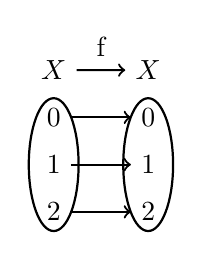
\begin{tikzpicture}[thick, scale=0.3]
  \draw (-2,0) ellipse [x radius=30pt, y radius=80pt];
  \draw (2,0) ellipse [x radius=30pt, y radius=80pt];
  \node[thick] (A) at (-2, 4) {$X$};
  \node[thick] (B) at (2,4) {$X$};
  \draw[thick, ->] (A) to  (B);

  
  \node[thick] (C) at (-2,2) {0};
   \node[thick] (D) at  (2,2) {0};

  
  \node[thick] (E) at (-2,0) {1};
  \node[thick] (F) at (2,0) {1};

    \node[thick] (G) at (-2,-2) {2};
    \node[thick] (H) at (2,-2) {2};

    
\draw[thick, ->] (C) to  (D);
\draw[thick, ->] (E) to  (F);
\draw[thick, ->] (G) to  (H);

\draw (0,5) node {f};
\end{tikzpicture}

    \begin{Def}
    设$f:X\to Y$,如果$\forall x_1, x_2 \in X$, 只要$x_1 \neq x_2$,  就 有 $f(x_1) \neq f(x_2)$,   则称$f$为从$X$到$Y$的{\bfseries 单射}。
  \end{Def}
一个单射的例子:

  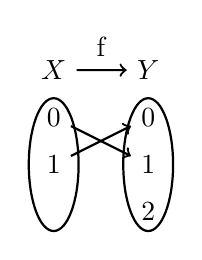
\begin{tikzpicture}[thick, scale=0.3]
  \draw (-2,0) ellipse [x radius=30pt, y radius=80pt];
  \draw (2,0) ellipse [x radius=30pt, y radius=80pt];
  \node[thick] (A) at (-2, 4) {$X$};
  \node[thick] (B) at (2,4) {$Y$};
  \draw[thick, ->] (A) to  (B);

  
  \node[thick] (C) at (-2,2) {0};
   \node[thick] (D) at  (2,2) {0};

  
  \node[thick] (E) at (-2,0) {1};
  \node[thick] (F) at (2,0) {1};

%    \node[thick] (G) at (-2,-2) {2};
    \node[thick] (H) at (2,-2) {2};

    
\draw[thick, ->] (C) to  (F);
\draw[thick, ->] (E) to  (D);
%\draw[thick, ->] (G) to  (H);

\draw (0,5) node {f};
\end{tikzpicture}

单射的符号化表示:

$f:X\to Y$

$\forall x1 \in X \forall x2 \in X x1 \neq x2 \to f(x1) \neq f(x2)$

即:$\forall x1 \in X \forall x2 \in X  f(x1) = f(x2) \to x1 = x2 $


  
  \begin{Def}
    设$f:X\to Y$, 如果$\forall y \in Y$, $\exists x \in X$使得 $f(x) = y$, 则称$f$为从$X$到$Y$的{\bfseries 满射}。
  \end{Def}

  一个满射的例子:

  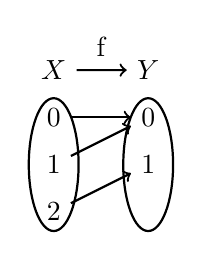
\begin{tikzpicture}[thick, scale=0.3]
  \draw (-2,0) ellipse [x radius=30pt, y radius=80pt];
  \draw (2,0) ellipse [x radius=30pt, y radius=80pt];
  \node[thick] (A) at (-2, 4) {$X$};
  \node[thick] (B) at (2,4) {$Y$};
  \draw[thick, ->] (A) to  (B);

  
  \node[thick] (C) at (-2,2) {0};
   \node[thick] (D) at  (2,2) {0};

  
  \node[thick] (E) at (-2,0) {1};
  \node[thick] (F) at (2,0) {1};

    \node[thick] (G) at (-2,-2) {2};
%    \node[thick] (H) at (2,-2) {2};

    
\draw[thick, ->] (C) to  (D);
\draw[thick, ->] (E) to  (D);
\draw[thick, ->] (G) to  (F);

\draw (0,5) node {f};
\end{tikzpicture}

满射的符号化表示:

$f:X\to Y$

$\forall y \in Y \exists x \in X f(x) = y$



  \begin{Def}
    设$f:X\to Y$,如果$f$既是单射又是满射,则称$f$为从$X$到$Y$的{\bfseries 双射},或者称$f$为从$X$到$Y$的一一对应。这时也称$X$与$Y${\bfseries 对等},记为$X\sim Y$。
  \end{Def}

  一个双射的例子:

  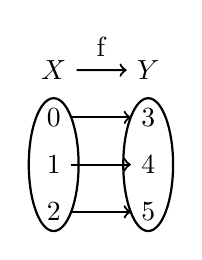
\begin{tikzpicture}[thick, scale=0.3]
  \draw (-2,0) ellipse [x radius=30pt, y radius=80pt];
  \draw (2,0) ellipse [x radius=30pt, y radius=80pt];
  \node[thick] (A) at (-2, 4) {$X$};
  \node[thick] (B) at (2,4) {$Y$};
  \draw[thick, ->] (A) to  (B);

  
  \node[thick] (C) at (-2,2) {0};
   \node[thick] (D) at  (2,2) {3};

  
  \node[thick] (E) at (-2,0) {1};
  \node[thick] (F) at (2,0) {4};

    \node[thick] (G) at (-2,-2) {2};
    \node[thick] (H) at (2,-2) {5};

    
\draw[thick, ->] (C) to  (D);
\draw[thick, ->] (E) to  (F);
\draw[thick, ->] (G) to  (H);

\draw (0,5) node {f};
\end{tikzpicture}

  \begin{Def}
    从集合$X$到集合$Y$的所有映射之集记为$Y^X$,即$\{f|f:X\to Y\}$。
  \end{Def}

  
$\{2,3\}^{\{0,1\}} = \{\{(0,2),(1,2)\},\{(0,3),(1,3)\},\{(0,2),(1,3)\},\{(0,3),(1,2)\}\}$

    \begin{Thm}[抽屉原理]
    如果把$n+1$个物体放到$n$个盒子里,则必有一个盒子里至少放了两个物体。
  \end{Thm}
  \begin{Example}
    从$1,2,\ldots, 2n$中任意选出$n+1$个数,则这$n+1$个数中必有两个数,使得其中之一能除尽另一个。
  \end{Example}
  \begin{proof}[证明]
  每个整数均可写成$2^l\cdot d$的形式,其中$l$为非负整数,$d$为奇数。因此,当把选出的$n+1$个整数都写成这种形式时,便得到了$n+1$个奇数$d_1,d_2,\cdots, d_{n+1}$,并且$1\leq d_i \leq 2n -1$,$i=1,2,\cdots, n+1$。但$1$到$2n$之间仅有$n$个奇数,由抽屉原理可知,必有$i,j$使得$d_i=d_j$,$i\neq j$。于是,$d_i$与$d_j$对应的两个整数$2^{l_i}\cdot {d_i}$与$2^{l_j}\cdot {d_j}$中必有一个可以整除另外一个。
  \end{proof}

 \begin{Example}
    任何6个人中,或有$3$个人互相认识,或有$3$个人互相不认识。
  \end{Example}

    \begin{Thm}[抽屉原理的强形式]
    设$q_1$,$q_2$,$\ldots$,$q_n$为$n$个正整数。如果把 $q_1 + q_2 + \cdots + q_n$  $- n$ $ + 1$ 个物体放到$n$个盒子中,则或者第一个盒子中至少含有$q_1$个物体,或者第二个盒子中至少含有$q_2$个物体,$\ldots$,
    或者第$n$个盒子中至少含有$q_n$个物体。
  \end{Thm}
  \begin{Cor}
    如果把$n(r-1) + 1$个物体放入$n$个盒子里,则至少有一个盒子里放了不少于$r$个物体。
  \end{Cor}
  \begin{Cor}
    如果$n$个正整数$m_1, m_2, \ldots, m_n$的平均值\[\frac{m_1 + m_2 + \ldots + m_n}{n} > r - 1,\] 则$m_1, m_2, \ldots, m_n$中至少有一个正整数不小于$r$。
  \end{Cor}
 
  \begin{Example}
    $n^2+1$个士兵站成一排,则可以使其中的至少$n+1$个士兵向前走一步站成一个按身高从小到大的队列,或站成一个按身高从大到小的队列。
  \end{Example}

  
  对照以下的例子可以帮助我们理解证明过程。

    \begin{tabular}{cccccccccc}
5& 9& 10& 4& 7& 2& 8& 3& 6& 1\\
3& 2& 1&  3& 2& 3& 1& 2& 1& 1\\
  \end{tabular}

  \begin{proof}[证明]
    从左到右依次用$h_1, h_2, \cdots, h_{n^2+1}$表示此队列中各士兵的身高,于是,我们得到了一个$n^2+1$项的数列
    \begin{equation}\label{soldier}
      h_1,h_2,\cdots, h_{n^2+1}
    \end{equation}
    我们的问题就是要证明此数列中或者有一个长(项数)至少为$n+1$的不减子序列,或者有一个长至少为$n+1$的不增子序列。

    假设本题结论不成立,则数列\eqref{soldier}中每个不减子序列的长度至多为$n$,每个不增子序列的长度也至多为$n$。令$m_i$为以$h_i$为首项的\eqref{soldier}的最长不减子序列的长度,$i=1,2,\cdots, n^2+1$。于是得到$n^2+1$个数$m_1,m_2,\cdots,m_{n^2+1}$,其中每个数$m_i$满足$1\leq m_i \leq n$。现在把这$n^2+1$个数放到$n$个盒子$1,2,\cdots,n$中,数$m_i$放到第$k$个盒子中当且仅当$m_i=k$,则必有某个盒子中至少含有$n+1$个数。由上述方法可知,在这同一个盒子中的至少$n+1$个数,它们是相等的。设这些数为$m_{i_1},m_{i_2},\cdots, m_{i_k}$,$i_1<i_2<\cdots<i_k\leq n^2+1$,$k>n$。相应的,我们有\eqref{soldier}的子序列
    \begin{equation}\label{subseq}
    h_{i_1}, h_{i_2}, \cdots, h_{i_k}      
    \end{equation}
    这是一个不增子序列。实际上,如若不然,例如$h_{i_1} < h_{i_2}$,则由于以$h_{i_2}$为首项的最长不减子序列的长为$m_{i_2}$,所以前面加一项$h_{i_1}$,就得到了一个以$h_{i_1}$为首项长度大于$m_{i_1}$的不减子序列,这是不可能的。

    于是,我们得到了一个长度至少为$n+1$的不增子序列\eqref{subseq},这又与假设相矛盾。所以,本题结论成立。
  \end{proof}
  \begin{Exercise}\justifying\let\raggedright\justifying
    设$a_1, a_2, \cdots, a_n$为$n$个实数且$a_1<a_2<\cdots <a_n$。$\varphi$为从$A=\{a_1,a_2,\cdots,a_n\}$ 到$A$的一一对应。试证:如果$a_1+\varphi(a_1)<a_2+\varphi(a_2)<\cdots < a_n+\varphi(a_n)$,则$\varphi = I_A$。
   \end{Exercise}
  \begin{proof}[证明]
    设$\varphi(a_1)\neq a_1$,则由$\varphi$为双射知存在$j$,$j>1$,$\varphi(a_j)=a_1$。于是,对任意的正整数$i<j$,$a_i+\varphi(a_i)<a_j+\varphi(a_j)=a_j+a_1$,由$a_i\geq a_1$知$\varphi(a_i)< a_j$,从而$\varphi(a_i)=a_k,k<j$。于是,对任意的$i$,$i<j$,$\varphi(a_i)\in \{a_2,\ldots,a_{j-1}\}$,由鸽笼原理,必存在$i_1<i_2<j$,$\varphi(i_1)=\varphi(i_2)$,这与$\varphi$为双射矛盾。类似可证,$\varphi(a_2)=a_2,\ldots,\varphi(a_n)=a_n$,即$\varphi = I_A$。
  
  \end{proof}
    \begin{Exercise}
    在一个半径为$16$的圆内任意放入$650$个点。给你一个形似垫圈的圆环,此圆环的外半径为$3$,内半径为$2$。现在要求你用这个垫圈盖住这$650$个点中的至少$10$个点,这可能吗?证明你的结论。
  \end{Exercise}
\begin{proof}[答]
  用这个垫圈可以盖住$650$个点中的至少$10$个点。以圆内的650个点中的每个点为圆心放一个圆环,则所有圆环的面积之和为$S_1 = 650 * \pi * (3^2 - 2^2) = 3250\pi$。所有圆环所覆盖的区域被包含在一个面积为$\pi * (16 + 3)^2= 361\pi$的圆$C$内。此时必存在$10$个圆环$R_1,R_2,\ldots, R_{10}$有公共的重叠区域,否则所有圆环的面积之和$S_1$将小于圆$C$之面积的$9$倍,即$3250\pi < 9 * 361\pi = 3249\pi$,矛盾。任取圆环$R_1,R_2,\ldots, R_{10}$的公共重叠区域中的一点,在该点上放一个圆环,将覆盖住$R_1,R_2,\ldots,R_{10}$的圆心,这$10$个圆心都是圆内$650$个点中的点,结论得证。 
\end{proof}



  
  \begin{Def}
    设$f:X\to Y$,$A \subseteq X$,$A$在$f$下的{\bfseries 象}定义为\[f(A)=\{f(x)|x\in A\}\]
  \end{Def}
  \begin{Example}
    设$f:\{-1,0,1\}\to \{0,1,2\}$,$f(x)=x^2$,则$f(\{-1,0\})=\{0,1\}$
  \end{Example}
  \begin{Def}
    设$f:X\to Y$,$B \subseteq Y$,$B$在$f$下的{\bfseries 原象}定义为\[f^{-1}(B)=\{x\in X|f(x)\in B\}\]
  \end{Def}
  \begin{Example}
    设$f:\{-1,0,1\}\to \{0,1,2\}$,$f(x)=x^2$,则$f^{-1}(\{1,2\})=\{-1,1\}$
  \end{Example}
  \begin{Thm}
    设$f:X\to Y$,$C \subseteq Y$,$D \subseteq Y$, 则
    \begin{enumerate}
    \item $f^{-1}(C \cup D) = f^{-1}(C) \cup f^{-1}(D)$
    \item $f^{-1}(C \cap D) = f^{-1}(C) \cap f^{-1}(D)$
    \item $f^{-1}(C \setminus D)=f^{-1}(C) \setminus f^{-1}(D)$
    \item $f^{-1}(C^c) = (f^{-1}(C))^c$
    \item $f^{-1}(C \bigtriangleup D) = f^{-1}(C) \bigtriangleup f^{-1}(D)$
    \end{enumerate}
  \end{Thm}
    \begin{Thm}
    设$f:X\to Y$,$A \subseteq X$,$B \subseteq X$, 则
    \begin{enumerate}
    \item $f(A \cup B) = f(A) \cup f(B)$
    \item $f(A \cap B) \subseteq f(A) \cap f(B)$
    \item $f(A \setminus B) \supseteq f(A) \setminus f(B)$
    \item $f(A \bigtriangleup B) \supseteq f(A) \bigtriangleup f(B)$
    \end{enumerate}
  \end{Thm}

  \begin{Def}
    设$f:X\to Y$,$g:Y\to Z$为映射,映射$f$与$g$的{\bfseries 合成}$g\circ f:X\to Z$定义为\[(g\circ f)(x) = g(f(x))\]
  \end{Def}
\begin{Thm}
  设$f:X \to Y$,$g:Y\to Z$,$h:Z\to W$ 为映射,则 \[ (h \circ g) \circ f = h \circ (g \circ f) \]
\end{Thm}
\begin{Thm}
  设$f:X \to Y$,则$f = f\circ I_X = I_Y \circ f$。
\end{Thm}
  \begin{Def}
     设$f:X\to Y$为双射,$f$的{\bfseries 逆映射}$f^{-1}:Y\to X$定义为:对任意的$y\in Y$,存在唯一的$x$使得$f(x)=y$,则$f^{-1}(y)=x$。
   \end{Def}

   \begin{Def}\label{inverse1}
          设$f:X\to Y$为一个双射, 则$g:Y\to X, g=\{(y,x)|(x,y)\in f\}$称为$f$的{\bfseries 逆映射},记为$g=f^{-1}$。
   \end{Def}
   \begin{Example}
     设集合$X=\{1,2,3\}$,$Y=\{4,5,6\}$,$f=\{(1,4),(2,5),(3,6)\}$为从$X$到$Y$的双射,则$f^{-1}=\{(4,1),(5,2),(6,3)\}$。
   \end{Example}
    \begin{Def}\label{inverse2}
     设$f:X\to Y$为一个映射。如果存在一个映射$g:Y\to X$使得\[f\circ g = I_{Y} \text{且} g\circ f = I_{X},\]则称映射$f$为{\bfseries 可逆}的,而$g$称为$f$的{\bfseries 逆映射}。
   \end{Def}
      \begin{Example}
     设集合$X=\{1,2,3\}$,$Y=\{4,5,6\}$,$f=\{(1,4),(2,5),(3,6)\}$为从$X$到$Y$的双射,$g=\{(4,1),(5,2),(6,3)\}$,由于$f\circ g = I_{Y}$且$ g\circ f = I_{X}$,$f^{-1}=g$。
   \end{Example}
\begin{Thm}
   定义\ref{inverse1}和定义\ref{inverse2}是等价的。
 \end{Thm}
 \begin{proof}[证明]
   设$f$为从集合$X$到集合$Y$的映射,$g$为从集合$Y$到集合$X$的映射。

   以下先假设$g$满足定义\ref{inverse1},往证$g$满足定义\ref{inverse2}。

   假设$f$为从集合$X$到集合$Y$的双射,$g$为从集合$Y$到集合$X$的映射,$g=\{(y,x)|(x,y)\in f\}$,则$(y,x)\in g$等价于$(x,y)\in f$,即$x=g(y)$等价于$y=f(x)$,易验证$f\circ g = I_{Y}$且$g\circ f = I_{X}$。

   接下来,假设$g$满足定义\ref{inverse2},往证$g$满足定义\ref{inverse1}。

   假设$f$为从集合$X$到集合$Y$的映射,存在一个映射$g:Y\to X$使得$f\circ g = I_{Y}$且$g\circ f = I_{X}$,往证$f$为双射,且$g=\{(y,x)|(x,y)\in f\}$。

   对任意的$x_1\in X$,$x_2\in X$,如果$f(x_1)=f(x_2)$,则$g(f(x_1))=g(f(x_2))$,再由$g\circ f = I_{X}$知$x_1=x_2$,从而$f$为单射。对任意的$y\in Y$,由$f\circ g = I_{Y}$知$f(g(y))=y$,从而$f$为满射。这证明了$f$为双射。

   以下证明$g=\{(y,x)|(x,y)\in f\}$,这就是要证$(y,x)\in g$等价于$(x,y)\in f$,即要证$x=g(y)$等价于$y=f(x)$。如果$x=g(y)$,则$f(x)=f(g(y))$,由$f\circ g=I_Y$知$y=f(x)$;如果$y=f(x)$,则$g(y)=g(f(x))$,由$g\circ f=I_X$知$x=g(y)$。

   %对任意的$(y,x)\in g$,则$x=g(y)$,从而$f(x)=f(g(y))$,由$f\circ g = I_{Y}$知$f(x)=y$,从而$(x,y)\in f$。

   %对任意的$(x,y)\in f$,则$y=f(x)$,从而$g(y)=g(f(x))$,由$g\circ f = I_{X}$知$g(y)=x$,从而$(y,x) \in g$。
 \end{proof}
 \begin{Thm}
    设$f:X\to Y$为可逆映射,则$(f^{-1})^{-1}=f$。
  \end{Thm}
  \begin{Thm}
    设$f:X\to Y$,$g:Y\to Z$都为可逆映射,则$g\circ f$也为可逆映射并且$(g\circ f)^{-1} = f^{-1}\circ g^{-1}$。
  \end{Thm}

    \begin{Def}
    设$f:X\to Y$为一个映射,如果存在一个映射 $g:Y\to X$ 使 得 $g\circ f = I_X$,
    则称$f$为左可逆的,$g$称为$f$的左逆映射;如果存在一个映射
    $h:Y\to X$ 使 得 $f\circ h=I_Y$,则称$f$为右可逆的,$h$称为$f$的右逆映射。
  \end{Def}
  \begin{Thm}
    设$f:X\to Y$为一个映射,则
    \begin{enumerate}
    \item $f$左可逆当且仅当$f$为单射;
    \item $f$右可逆当且仅当$f$为满射。
    \end{enumerate}
  \end{Thm}
  \begin{proof}[证明]
    先证(1)。

设$f$为左可逆的,则存在一个映射 $g:Y\to X$ 使 得 $g\circ f = I_X$。对任意的$x_1\in X$,$x_2\in X$,如果$f(x_1)=f(x_2)$,则$g(f(x_1))=g(f(x_2))$,再由$g\circ f = I_{X}$知$x_1=x_2$,从而$f$为单射。

设$f$为单射,则$f$为从集合$X$到$Im(f)$的双射。于是,存在$g:Im(f)\to X$使得$g\circ f = I_X$。扩充$g$到$Y$上:对任意的$y\in Y$,若$y\in  Im(f)$,则$g(y)$不变,而当$y\in Y\setminus Im(f)$时,规定$g(y)$为$X$中任意一个固定的元素$x_0$,则$g$为从集合$Y$到集合$X$的映射,且$g\circ f = I_X$。所以,$f$为左可逆的。

再证(2)。

设$f$为右可逆的,则存在一个映射$g:Y\to X$ 使 得 $f\circ g=I_Y$。对任意的$y\in Y$,由$f\circ g = I_{Y}$知$f(g(y))=y$,从而$f$为满射。

设$f$为满射,则对任意的$y\in Y$,$f^{-1}(\{y\})\neq \phi$。令$g:Y\to X$,其定义为,对任意的$y\in Y$,$g(y)=x$,其中$x$为$f^{-1}(\{y\})$中一个特定元素。于是,对任意的$y\in Y$,设$g(y)=x$,则$f(x)=y$,从而$(f\circ g)(y) = f(g(y)) = f(x) = y = I_Y(y)$。所以$f\circ g=I_Y$,即$f$为右可逆的。
  \end{proof}

  \begin{Def}
    有穷集合$S$到自身的一一对应称为$S$上的一个置换。如果$|S| = n$, 则$S$上的置换就说成是$n$次置换。
  \end{Def}
设$S=\{1,2,\ldots,n\}$,$\sigma:S\to S$为$S$上的一个置换,$\sigma(1) = k_1$, $\sigma(2) = k_2$,$\ldots$,$\sigma(n) = k_n$,我们用如下的一个表来表示置换$\sigma$:
\[\sigma=\begin{pmatrix}1&2&\ldots&n\\k_1&k_2&\ldots&k_n\end{pmatrix}\]
$S$上所有的$n$次置换构成的集合记为$S_n$。
\begin{Example}
  设$S=\{1,2,3,4\}$,$\sigma:S\to S$,$\sigma(1) = 3$, $\sigma(2) = 2$, $\sigma(3) = 4$, $\sigma(4) = 1$,则$\sigma$可以表示为
  \[\sigma=\begin{pmatrix}1&2&3&4\\3&2&4&1\end{pmatrix}\]
  这里,列的次序无关紧要,例如,$\sigma$还可以表示为
  \[\sigma=\begin{pmatrix}2&1&3&4\\2&3&4&1\end{pmatrix}\]
\end{Example}

  \begin{Def}
    设$\alpha$与$\beta$为集合$S$上的两个置换,则$\alpha$与$\beta$为两个从$S$到$S$的双射,讨论置换时,我们用$\alpha\beta$表示$\alpha$与$\beta$的合成$\beta \circ \alpha$。
    注意这里$\alpha$与$\beta$的次序,从运算的角度看有一定的便利性,但也有的教材中采用相反的顺序。按照我们的写法,讨论置换时,如果$i \in S$,则用$(i)\alpha$表示$i$在$\alpha$下的像,简记为$i\alpha$。
  \end{Def}
  \begin{Example}
    设$S=\{1,2,3\}$,$\alpha$和$\beta$为$S$上的两个置换,
    \[\alpha=\begin{pmatrix}1&2&3\\1&3&2\end{pmatrix},\beta=\begin{pmatrix}1&2&3\\2&3&1\end{pmatrix}\],
    则
    \[\alpha\beta=\begin{pmatrix}1&2&3\\1&3&2\end{pmatrix}\begin{pmatrix}1&2&3\\2&3&1\end{pmatrix}=\begin{pmatrix}1&2&3\\2&1&3\end{pmatrix}\],    
  \end{Example}

   若$\alpha$与$\beta$为两个$n$次置换,当把$\beta$的表示式中的上一行按$\alpha$的下一行的顺序写出时,则$\alpha \beta$的下一行就是$\beta$的新表示式中的下一行。
  \begin{Example}
    设$S=\{1,2,3\}$,$\alpha$和$\beta$为$S$上的两个置换,
    \[\alpha=\begin{pmatrix}1&2&3\\1&3&2\end{pmatrix},\beta=\begin{pmatrix}1&2&3\\2&3&1\end{pmatrix}\],
    则
    \[\alpha\beta=\begin{pmatrix}1&2&3\\1&3&2\end{pmatrix}\begin{pmatrix}1&2&3\\2&3&1\end{pmatrix}=\begin{pmatrix}1&2&3\\1&3&2\end{pmatrix}\begin{pmatrix}1&3&2\\2&1&3\end{pmatrix}=\begin{pmatrix}1&2&3\\2&1&3\end{pmatrix}\],    
  \end{Example}   
   \begin{Def}
     设$\sigma$为$S$上的一个$n$次置换,若$i_1\sigma=i_2$,$i_2\sigma = i_3$, $\cdots$, $i_{k-1}\sigma = i_k$, $i_k\sigma = i_1$,而$\forall i \in S\setminus \{i_1, i_2, \ldots, i_k\}$, $i\sigma = i$,
     则称$\sigma$为一个$k$循环置换,记为$(i_1i_2\cdots i_k)$。 $2-$循环置换称为对换。
   \end{Def}
   \begin{Example}
   设$S=\{1,2,3,4,5\}$,则\[(1 2 3)=\begin{pmatrix}1&2&3&4&5\\2&3&1&4&5\end{pmatrix},(2 3)=\begin{pmatrix}1&2&3&4&5\\1&3&2&4&5\end{pmatrix}\]     
   \end{Example}
   \begin{Thm}
    每个置换都能被分解成若干个没有共同数字的循环置换的乘积。如果不计这些循环置换的顺序以及略去的$1-$循环置换,这个分解是唯一的。
   \end{Thm}
   \begin{Thm}
    当$n\geq 2$时,每个$n$次置换都能被分解成若干个对换的乘积。
   \end{Thm}
   \begin{Thm}
    如果把置换分解成若干个对换的乘积,则对换个数的奇偶性是不变的。
  \end{Thm}
  \begin{proof}[证明]
    设$\sigma$为一个$n$次置换。$\sigma$的符号$sign(\sigma)$定义为$(-1)^{|\{(x,y)|x < y \land (x)\sigma^{-1} > (y)\sigma^{-1} \}|}$。

设$\alpha = \beta (i,j)$,则$sign(\alpha) = -sign(\beta)$。

于是,如果置换$\sigma$可以分解为$m$个对换的乘积$\sigma = I(i_1k_1)(i_2k_2)\cdots (i_mk_m)$,其中$I$为恒等置换,由$sign(I)=1$知$sign(\sigma) = (-1)^m$。而$sign(\sigma)$只能为$1$和$-1$两者之一,因此如果$\sigma$能分解成偶数个对换的乘积,则只能分解成偶数个对换的乘积;如果$\sigma$能分解成奇数个对换的乘积,则只能分解成奇数个对换的乘积。
  \end{proof}
  \begin{Def}
    能被分解为偶数个对换的乘积的置换称为偶置换;能被分解为奇数个对换的乘积的置换称为奇置换。
  \end{Def}
    \begin{Thm}
    当$n \geq 2$时, $n$次奇置换的个数与$n$次偶置换的个数相等,都等于$\frac{n!}{2}$。
  \end{Thm}
     \begin{proof}[证明]
     设$A$为所有的$n$次奇置换所构成的集合,$B$为所有的$n$次偶置换所构成的集合,则$S_n=A\cup B$且$A\cap B=\phi$。所以,$|S_n|=|A| + |B|=n!$。

     以下证明$|A|=|B|$。构造映射$f:A\to B$,对任意的$\sigma\in A$,$f(\sigma) = \sigma(12)$。易验证$f$为单射,这是因为对任意的$\sigma_1\in A$,$\sigma_2\in A$,如果$f(\sigma_1)=f(\sigma_2)$,则$\sigma_1(12)=\sigma_2(12)$,从而$\sigma_1(12)(12)=\sigma_2(12)(12)$,即$\sigma_1=\sigma_2$。同时,易验证$f$为满射,这是因为对任意的$\tau \in B$,$f(\tau(12))=\tau(12)(12)=\tau$。从而$f$为双射,这证明了$|A|=|B|$。再由$|A|+|B|=n!$知,$|A|=|B|=\frac{n!}{2}$。
   \end{proof}

      \begin{Def}
    一个集合及其在该集合上定义的若干个代数运算合称为一个代数系。
  \end{Def}
  我们熟知的实数集$R$,与其上的加法运算"$+$"和乘法运算"$*$"一起构成了一个代数系,满足如下性质:
  
    设$x, y, z \in \mathbb{R}$,则
   \begin{enumerate}
   \item   $x + y = y + x$
   \item   $(x + y) + z = x + (y + z)$
   \item   $0 + x = x + 0 = x$
   \item   $(-x) + x =x + (-x) = 0$
   \item   $x * y = y * x$
   \item   $(x * y) * z = x * (y *z)$
   \item   $1 * x = x * 1 = x$
   \item   $x^{-1} * x = x * x^{-1} = 1 (x \neq 0)$
   \item   $x* (y + z) = x * y + x * z$
   \item   $(y + z) * x = y * x + z * x$
    \end{enumerate}

  %   在实数集$R$上还定义了小于关系$<$,满足如下性质:
       

  % \begin{enumerate}
  % \item 对任意的$x\in R$,$y\in R$,$x<y$,$x=y$,$y<x$中有且仅有一个成立。 
  % \item 对任意的$x\in R$,$y\in R$,$z\in R$,如果$x<y$并且$y<z$,则$x<z$。
  % \item 对任意的$x\in R$,$y\in R$,$z\in R$,如果$x<y$,则$x+z<y+z$。
  % \item 对任意的$x\in R$,$y\in R$,如果$x>0$,$y>0$,则$xy>0$。
  % \end{enumerate}

  % 另外,实数集还具有如下性质:

  % 设$A_1$, $A_2$,$\cdots$,$A_i$,$\cdots$为实数集$R$上的闭区间,$A_1\supseteq A_2 \supseteq A_3 \supseteq \cdots \supseteq A_i \supseteq \cdots$,则$\bigcap_{i=1}^{\infty}A_i$非空。
  \begin{Def}
    设$X$,$Y$,$Z$为任意三个非空集合。一个 从 $X\times Y$到$Z$的映射 $\phi$ 称 为 $X$与$Y$到$Z$的一个二元(代数)运算。当$X=Y=Z$时,则称$\phi$为$X$上的二元(代数)运算。
  \end{Def}
  \begin{Def}
    从集合$X$到$Y$的任一映射称为从$X$到$Y$的一元(代数)运算。如果$X=Y$,则从$X$到$X$的映射称为$X$上的一元(代数)运算。
  \end{Def}
  \begin{Def}
    设$A_1, A_2, \cdots, A_n, D$为非空集合。一个从 $A_1\times A_2\times \cdots \times A_n$到$D$的映射$\phi$称为$A_1, A_2, \cdots, A_n$到$D$的一个$n$元(代数)运算。
    如果$A_1=A_2=\cdots=A_n=D=A$,则称$\phi$为$A$上的$n$元代数运算。
  \end{Def}

  \begin{Def}
    设“$\circ$”为集合$X$上的一个二元代数运算。如果$\forall a, b \in X$,恒有\\$a \circ b = b \circ a$, 则称二元代数运算“$\circ$”满足交换律。
  \end{Def}
  \begin{Def}
    设“$\circ$”为集合$X$上的一个二元代数运算。如果$\forall a, b, c \in X$,恒有$(a \circ b) \circ c = a \circ (b \circ c)$, 则称二元代数运算“$\circ$”满足结合律。
  \end{Def}
  \begin{Def}
    设“$+$”与“$\circ$”为集合$X$上的两个二元代数运算。\\如果$\forall a, b, c \in X$,恒有\[a \circ (b + c) = a \circ b + a \circ c,\] 则称二元代数运算“$\circ$”对“$+$”满足左分配律。
    如果$\forall a, b, c \in X$,恒有\[(b + c)\circ a = b \circ a + c \circ a,\] 则称二元代数运算“$\circ$”对“$+$”满足右分配律。
  \end{Def}
  \begin{Def}
    设$(X, \circ)$为一个代数系。如果存在一个元素$e\in X$使得对任意的$x\in X$恒有$e\circ x = x \circ e = x$, 则称$e$为“$\circ$”的单位元素。
  \end{Def}
  \begin{Def}
    设$(X, \circ)$为一个代数系,“$\circ$”有单位元素$e$,$a\in X$,如果$\exists b\in X$使得\[a\circ b = b \circ a = e,\]  则称$b$为$a$的逆元素。
  \end{Def}
  \begin{Def}
    设$(S,+)$与$(T, \oplus)$为两个代数系。如果存在一个一一对应$\phi:S\to T$, 使得$\forall x, y \in S$,有
    \begin{align*}
      \phi(x+y) &= \phi(x) \oplus \phi(y),
    \end{align*}
    则称代数系$(S,+)$与$(T, \oplus)$同构,并记为$S\cong T$, $\phi$称为这两个代数系之间的一个同构。
  \end{Def}
  \begin{Def}
    设$(S,+, \circ)$与$(T, \oplus, *)$为两个代数系。如果存在一个一一对应$\phi:S\to T$, 使得$\forall x, y \in S$,有
    \begin{align*}
      \phi(x+y) &= \phi(x) \oplus \phi(y),\\
      \phi(x\circ y)&= \phi(x) * \phi(y),
    \end{align*}
    则称代数系$(S,+,\circ)$与$(T, \oplus, *)$同构,并记为$S\cong T$, $\phi$称为这两个代数系之间的一个同构。
  \end{Def}
  \begin{tabular}{cc|c}
    p& q& p $\land$ q\\
    \hline
    T&T&T\\
    T&F&F\\
    F&T&F\\
    F&F&F\\
  \end{tabular}\hspace{1cm}
  \begin{tabular}{cc|c}
    p& q& p $\lor$ q\\
    \hline
    T&T&T\\
    T&F&T\\
    F&T&T\\
    F&F&F\\
  \end{tabular}\hspace{1cm}
  \begin{tabular}{c|c}
    p& $\lnot$ p\\
    \hline
    T&F\\
    F&T\\
  \end{tabular}

  \vspace{1cm}
    \begin{tabular}{cc|c}
    x& y& x $\land$ y\\
    \hline
    1&1&1\\
    1&0&0\\
    0&1&0\\
    0&0&0\\
  \end{tabular}\hspace{1cm}
  \begin{tabular}{cc|c}
    x& y& x $\lor$ y\\
    \hline
    1&1&1\\
    1&0&1\\
    0&1&1\\
    0&0&0\\
  \end{tabular}\hspace{1cm}
  \begin{tabular}{c|c}
    x& $\bar{x}$\\
    \hline
    1&0\\
    0&1\\
  \end{tabular}
  
代数系$(\{T,F\},\land,\lor,\lnot)$与$(\{1,0\},\land, \lor,\bar{ })$是同构的。
  \begin{Def}
    设$X$为一个集合,$E \subseteq X$。 $E$的特征函数$\chi_E:X\to \{0,1\}$定义为
    \begin{equation*}
      \chi_E(x)=
      \begin{cases}
        1 & \text{如果} x \in E,\\
        0 & \text{如果} x \notin E.
      \end{cases}
    \end{equation*}
  \end{Def}
  \begin{Def}
    令$Ch(X) = \{\chi |\chi:X \to \{0,1\}\}$。
    $\forall \chi, \chi' \in Ch(X)$及$x \in X$,
    \begin{align}
      (\chi \lor \chi')(x) &= \chi(x) \lor \chi'(x)\nonumber\\
      (\chi \land \chi')(x) &= \chi(x) \land \chi'(x)\nonumber\\
      \bar{\chi}(x) &=   \overline{\chi(x)}
    \end{align}
  \end{Def}
  \begin{Thm}
    设$X$为一个集合,则代数系$(2^X, \cup, \cap, ^c)$与$(Ch(X), \lor, \land, \bar{} \ )$同构。
  \end{Thm}
  \begin{align*}
    X=\{&1,2,3\}\\
    2^X=\{&\\
        \phi,&\hspace{1.5cm}\chi_1:X\to \{0,1\}\hspace{0.5cm} \chi_1(1)=0,\chi_1(2)=0,\chi_1(3)=0\\
    \{1\},&\hspace{1.5cm}\chi_2:X\to \{0,1\}\hspace{0.5cm} \chi_2(1)=1,\chi_2(2)=0,\chi_2(3)=0\\
        \{2\},&\hspace{1.5cm}\chi_3:X\to \{0,1\}\hspace{0.5cm} \chi_3(1)=0,\chi_3(2)=1,\chi_3(3)=0\\
    \{3\},&\hspace{1.5cm}\chi_4:X\to \{0,1\}\hspace{0.5cm} \chi_4(1)=0,\chi_4(2)=0,\chi_4(3)=1\\
    \{1,2\},&\hspace{1.5cm}\chi_5:X\to \{0,1\}\hspace{0.5cm} \chi_5(1)=1,\chi_5(2)=1,\chi_5(3)=0\\
    \{2,3\},&\hspace{1.5cm}\chi_6:X\to \{0,1\}\hspace{0.5cm} \chi_6(1)=0,\chi_6(2)=1,\chi_6(3)=1\\
    \{1,3\},&\hspace{1.5cm}\chi_7:X\to \{0,1\}\hspace{0.5cm} \chi_7(1)=1,\chi_7(2)=0,\chi_7(3)=1\\
    \{1,2,3\}&\hspace{1.5cm}\chi_8:X\to \{0,1\}\hspace{0.5cm} \chi_8(1)=1,\chi_8(2)=1,\chi_8(3)=1\\
    \}\\
  \end{align*}

  \begin{Exercise}
    设$f:X\to Y$。试证:$f$为满射当且仅当对任意的$E\in 2^Y$,$f(f^{-1}(E))=E$。
    \end{Exercise}
    \begin{proof}[证明]
      设$f$为满射,对任意的$E\in 2^Y$往证$f(f^{-1}(E))=E$。
    
      对任意的$y$,$y\in f(f^{-1}(E))$,则存在$x$,$x\in f^{-1}(E)$并且$y=f(x)$,于是存在$x$,$f(x) \in E$并且$y=f(x)$,从而$y\in E$。
    
      对任意的$y$,$y\in E$,由$f$为满射知存在$x\in X$,$y=f(x)$,从而$f(x)\in E$,即$x\in f^{-1}(E)$,由$y=f(x)$知$y\in f(f^{-1}(E))$。
    
      设对任意的$E\in 2^Y$,$f(f^{-1}(E))=E$,往证$f$为满射。
    
      对任意的$y\in Y$,则$f(f^{-1}(\{y\}))=\{y\}$,于是$f^{-1}(\{y\})\neq \phi$,从而存在$x\in X$,$x\in f^{-1}(\{y\})$, 即$f(x)\in \{y\}$,等价的,$f(x)=y$,故$f$为满射。
    \end{proof}
    \begin{Exercise}
      设$f:X\to Y$。试证:$f$为单射当且仅当对任意的$F\in 2^Y$,$f^{-1}(f(F))=F$。
      \end{Exercise}
      \begin{proof}[证明]
        设$f$为单射,对任意的$F\in 2^Y$,往证$f^{-1}(f(F))=F$。
      
        对任意的$x$,$x\in f^{-1}(f(F))$,则$f(x)\in f(F)$,于是存在$x'\in F$,$f(x)=f(x')$,由$f$为单射知$x=x'$,从而$x\in F$。
      
        对任意的$x$,$x\in F$,则$f(x)\in f(F)$,从而$x\in f^{-1}(f(F))$。
      
        设对任意的$F\in 2^Y$,$f^{-1}(f(F))=F$,以下证明$f$为单射。
      
        对任意的$x_1\in X$,$x_2\in X$,如果$f(x_1)=f(x_2)$,则$f(\{x_1\})=f(\{x_2\})$,于是$f^{-1}(f(\{x_1\}))=f^{-1}(f(\{x_2\}))$,从而$\{x_1\}=\{x_2\}$,于是$x_1=x_2$。
        
      \end{proof}
  \clearpage     
  \begin{Exercise}
    试证:每个$n$次置换均可被分解成这样的一些置换的乘积:每个置换或为$(12)$,或为
    $(23\cdots n)$。  
    \end{Exercise}
    \begin{proof}[证明]
      \[(23\cdots n)^{-1}(12)(23\cdots n) = (13)\]
      \[(23\cdots n)^{-1}(13)(23\cdots n) = (14)\]
      $\ldots$
      \[(23\cdots n)^{-1}(1 n-1)(23\cdots n) = (1 n)\]
      每个置换均可被分解成(12),(13),$\cdots$,(1n)的乘积,故结论成立。
    \end{proof}

    \begin{Exercise}
      任一偶置换均可被分解成3-循环置换$(123)$,$(124)$,$\ldots$,$12n$中若干个之乘积。 
      \end{Exercise}
      \begin{proof}[证明]
        \[(12i)(12j)=(2i)(1j)\]
        \[(12s)(12t)=(2s)(1t)\]
        \[(12i)(12j)(12s)(12t)(12i)(12j)=(2i)(1j)(2s)(1t)(2i)(1j)=(2i)(2s)(2i)(1j)(1t)(1j)=(is)(jt)\]
      \end{proof}
      
        
  
  
\chapter{}

\end{CJK*}
\end{document}





%%% Local Variables:
%%% mode: latex
%%% TeX-master: t
%%% End:



